\section*{\centering Diffraktion i en spalt respektive en cirkulär apertur}
\section{Teori}
Detta avsnitt grundar sig på kapitel 33 i Tipler och Moscas bok \textit{Physics for Scientists and Engineers} (2008).
\vspace{5mm}

Vid Fraunhofer-diffraktion i enkelspalt ges diffraktionsvinkeln $\theta$ för minimum av ordning $m$ av

\begin{equation}
    \text{sin}(\theta) = \dfrac{m\lambda}{a},
\end{equation}

där $\lambda =$ våglängden och $a =$ spaltvidden. Ljusets intensitet i diffraktionsmönstret ges av följande ekvation:

\begin{equation}
    I(\theta) = I(0) \left( \dfrac{\text{sin}(\beta)}{\beta} \right)^{2}.
\end{equation}

$I(0) =$ den observerade intensiteten i centrum av mönstret $(\theta = 0)$. \\
$\beta = \dfrac{1}{2} k a \text{sin}(\theta)$, där $a =$ spaltvidden och $k = \dfrac{2\pi}{\lambda}$.
\vspace{5mm}

För en cirkulär öppning kan diffraktionsvinkeln för minimum av ordning $n$ beräknas med

\begin{equation}
    \text{sin}(\theta) = \dfrac{m\lambda}{D},
\end{equation}

där $D =$ öppningens diameter och $m$ är lika med 1.22, 2.23 och 3.24 för ordning $n=1$, $n=2$ respektive $n=3$. Intensiteten ges av nedanstående ekvation där $J_{1}$ är en Besselfunktion av första slaget.

\begin{equation}
    I(\theta) = I(0) \left( \dfrac{2J_{1}(\beta)}{\beta} \right)^{2}.
\end{equation}

$I(0) =$ den observerade intensiteten i centrum av mönstret $(\theta = 0)$. \\
$\beta = \dfrac{1}{2} k D \text{sin}(\theta)$, där $D =$ hålets diameter och $k = \dfrac{2\pi}{\lambda}$.

\section{Resultat}

\begin{figure}[H]
    \centering
    \captionsetup{justification=centering,margin=2cm}
    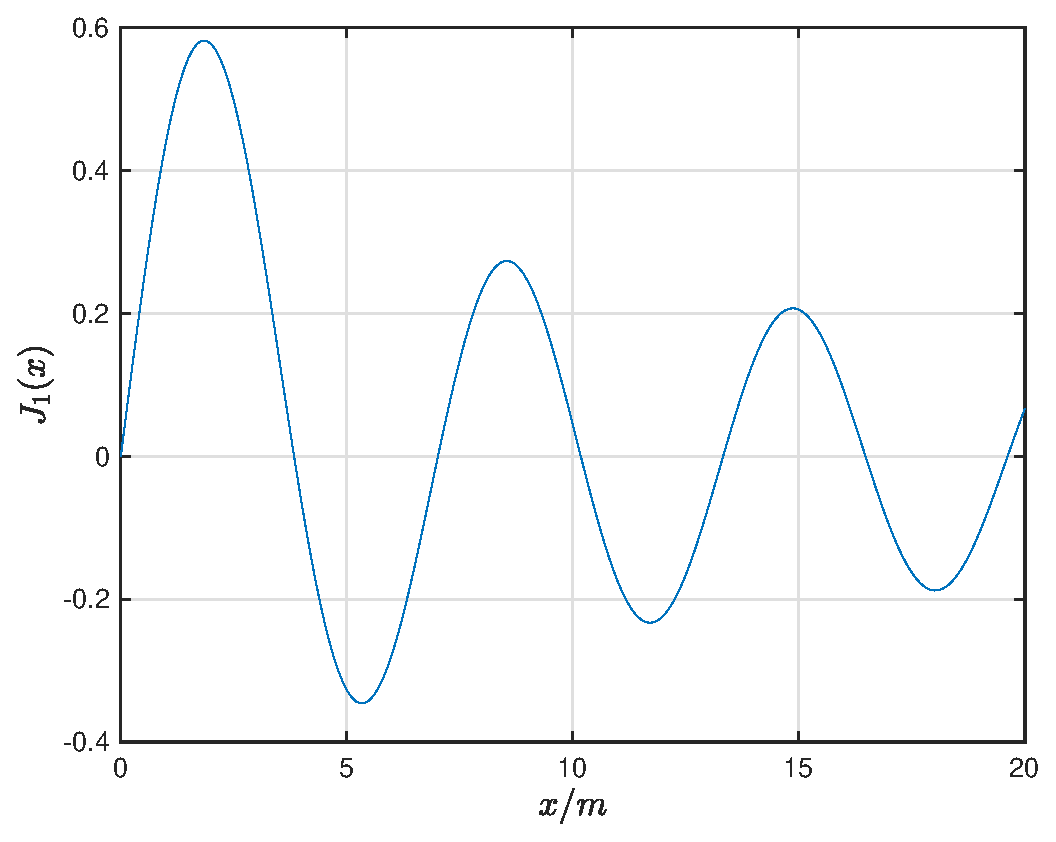
\includegraphics[scale=0.5]{Resources/Graphics/fig5_1.eps}
    \caption{Besselfunktion av första slaget.}
    \label{fig:5_1}
\end{figure}



\begin{figure}[H]
    \centering
    \captionsetup{justification=centering,margin=2cm}
    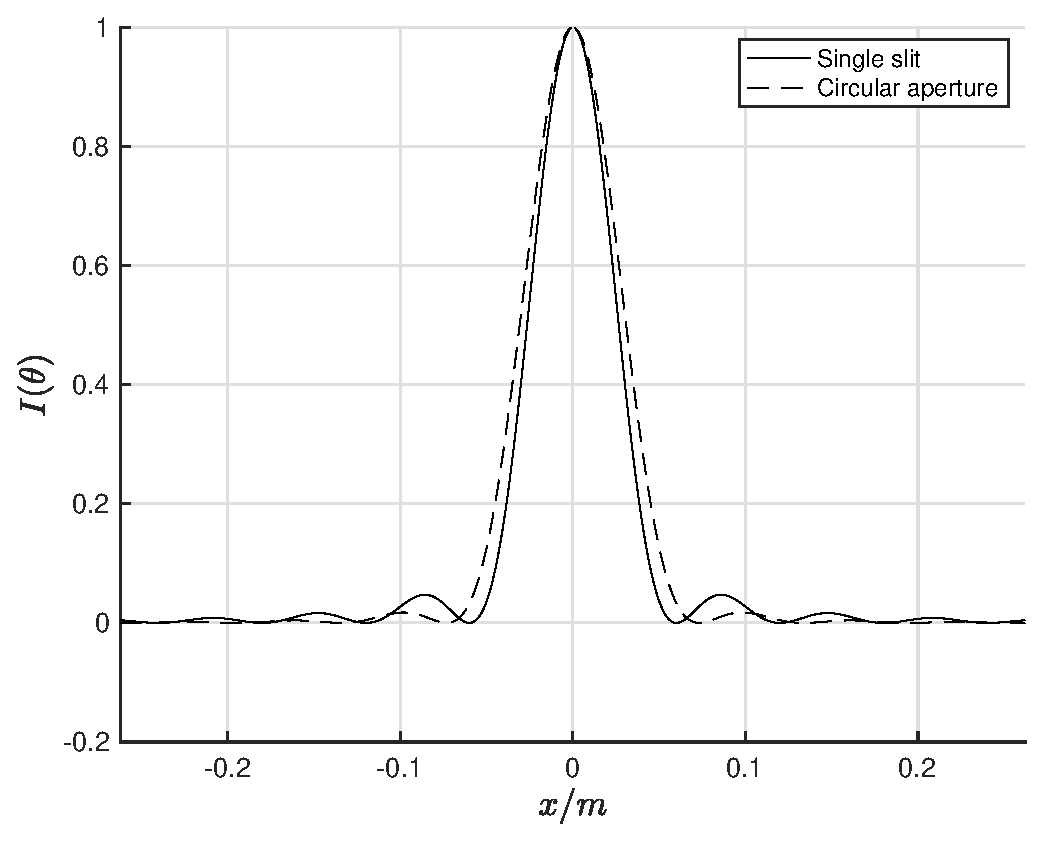
\includegraphics[scale=0.5]{Resources/Graphics/fig5_2.eps}
    \caption{Intensitetsprofil av Fraunhofer-mönster för enkelspalt (genomdragen kurva) och cirkulär öppning (streckad kurva).}
    \label{fig:5_2}
\end{figure}

\begin{figure}[H]
    \centering
    \captionsetup{justification=centering,margin=2cm}
    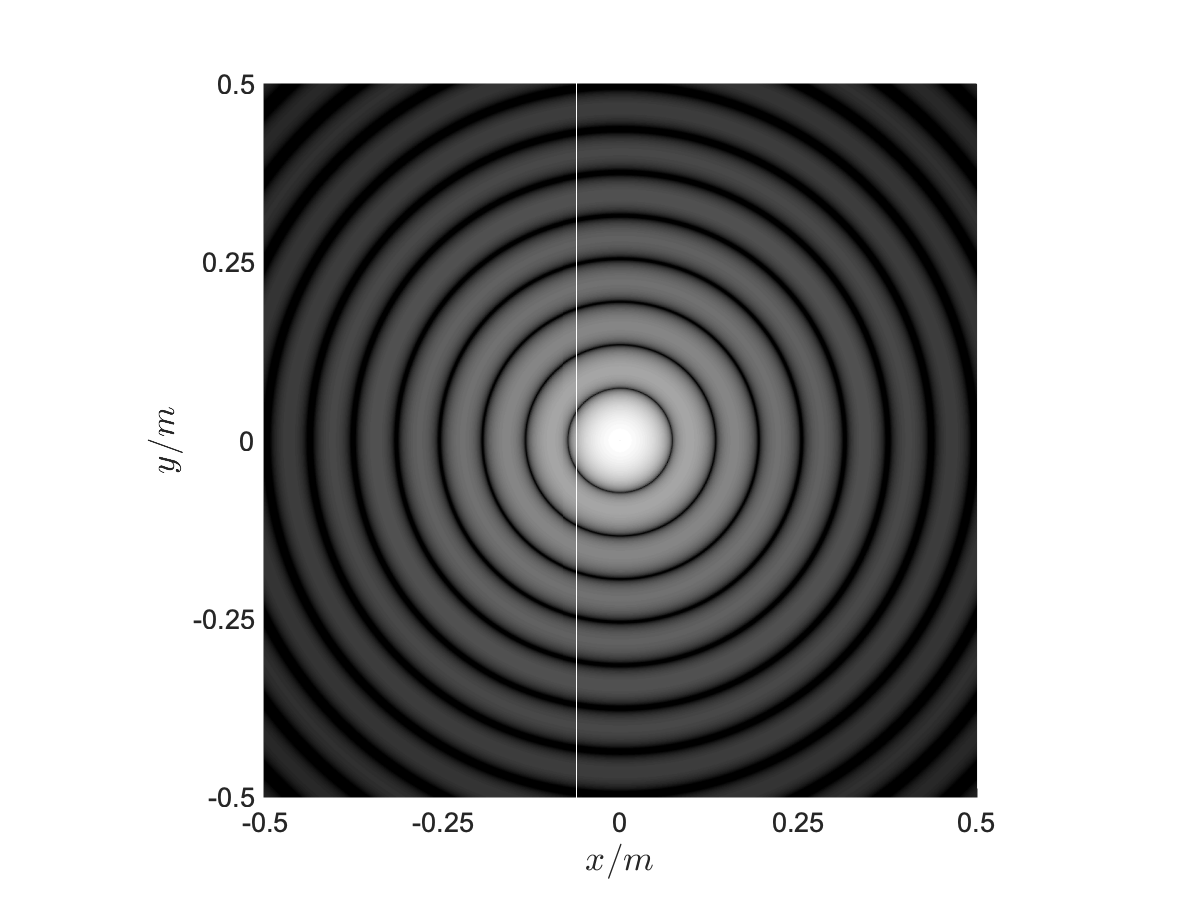
\includegraphics[scale=0.65]{Resources/Graphics/fig5_3.eps}
    \caption{Tvådimensionellt Fraunhofer-mönster för cirkulär öppning.}
    \label{fig:5_3}
\end{figure}

\begin{figure}[H]
    \centering
    \captionsetup{justification=centering,margin=2cm}
    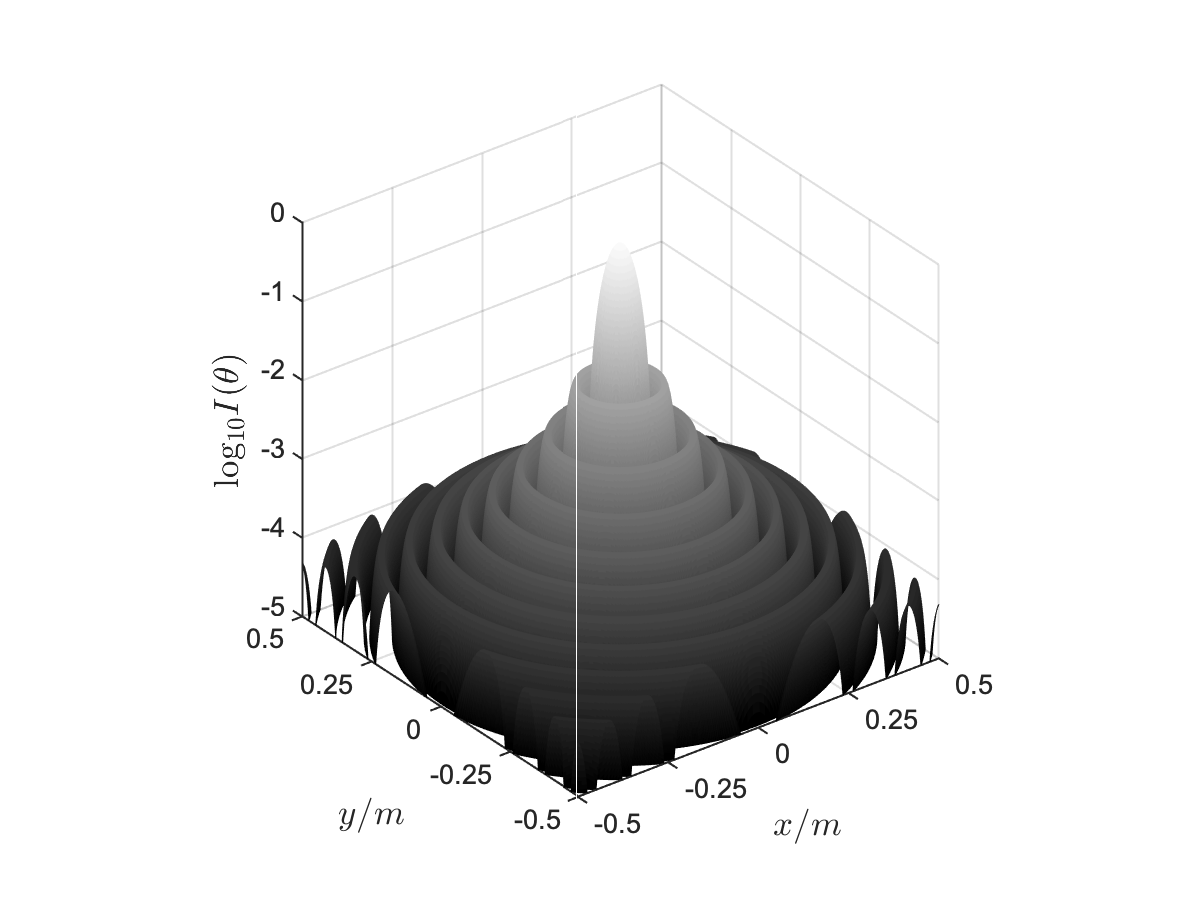
\includegraphics[scale=0.65]{Resources/Graphics/fig5_4.eps}
    \caption{Tredimensionellt Fraunhofer-mönster för cirkulär öppning.}
    \label{fig:5_4}
\end{figure}

\section{Diskussion}
Eftersom intensiteten vid diffraktion i cirkulär öppning ges av ekvation 4, går det i Figur 1 (Besselfunktionen) i x-axeln att avläsa $\beta$ för diffraktionsmönstrets sekundära minima samt maxima. Minima finnes vid nollställena och maxima vid kurvtopparna. I Figuren går att se att första sekundära maxima har störst intensitet (av alla sekundära maxima) och att intensiteten sedan avtar med ökande ordning. I både Figur 3 och 4 illustreras detta av de olika ljusa ringarna (maxima) samt de helt mörka ringarna (minima).

Av Figur 2 framgår det att intensitetsfördelningen för enkelspalten och den cirkulära öppningen är ganska lik men ändå skiljer sig åt på så vis att diffraktionsvinkeln för sekundära minima och maxima i fallet med den cirkulära öppningen är större än i fallet med enkelspalten, samt på så vis att sekundära maxima har lägre intensitet i det tidigare fallet. Anledningen till att intensitetsfördelningen är ganska lik för de båda fallen är rimligt i och med att spaltvidden är lika stor som diametern. Skillnaden kan förklaras dels med att sinusfunktionen i ekvation 2 ersatts med en Besselfunktion i fallet med den cirkulära öppningen, och dels med ekvation 3, där $m$ till skillnad från $m$ i ekvation 1 ökar med mer än 1 för varje ordning.

\subsection*{Referenser}
Mosca, Gene; Tipler, A., Paul. 2008. \textit{Physics for Scientists and Engineers}. 6:e upplagan. W.H. Freeman and Company, New York.

\np
\subsection*{MatLab-kod}
\lstinputlisting[caption={\quad},firstline=3] {Resources/Code/5.m}































